\section{Organisation}

% text d'intro ! 
	\subsection{Versions}
		Nous avons découpé le développement de \glasir{} en différentes versions, chacune incrémentale en fonctionnalités.
		Cela nous permettra de toujours avoir un produit fonctionnel, et facilitera les phases de tests.

		\begin{table}[h!]
			\begin{center}
			\begin{tabular}{|c|c|}
				\hline
				Version & Description\\
				\hline
				0.1 & Application qui lance ADTool\\
				\hline
				0.2 & Création d'un projet\\
				\hline
				0.3 & Paramètre de synthèse\\
				\hline
				0.4 & Filtre\\
				\hline
				0.5 & Optimiseur\\
				\hline
				0.6 & Bibliothèque de modèles\\
				\hline
				1.0 & Version pour la soutenance\\
				\hline
			\end{tabular}
			\end{center}
			\caption{Tableau regroupant nos versions}
		\end{table} % ajouter release date ? 

		Les améliorations sur ADTool seront réalisées en parallèle du développement de \glasir{}.

	\subsection{Planification}
		Une ébauche de la planification se trouve figure \ref{fig:planif}. Celle-ci donne un aperçu du temps de développement qui sera passé pour chaque version de \glasir{}. 

		\begin{landscape}
			\begin{figure}
				\centering
				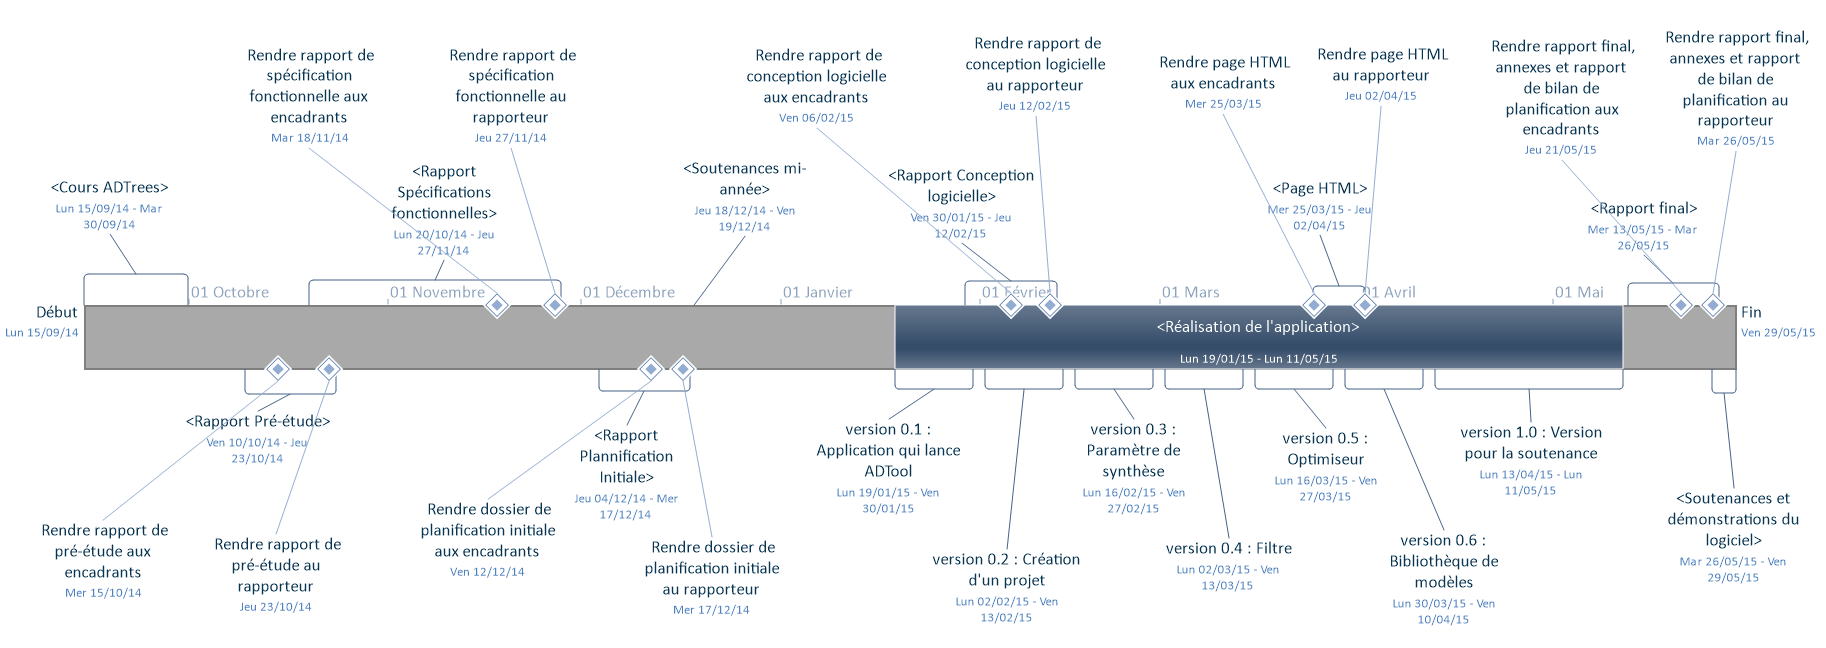
\includegraphics[height=0.50\textwidth]{figure/planification.png}
				\caption{Planif MS Project}
				\label{fig:planif}
			\end{figure}
		\end{landscape}


	\subsection{Répartition des tâches}
		Au second semestre, seuls resteront Pierre-Marie {\sc Airiau}, Valentin {\sc Esmieu} et Maud {\sc Leray} sur ce projet, étant donné que le reste du groupe part étudier à l'étranger. Par conséquent, nous comptons séparer le travail ainsi :
		\begin{itemize} % donner les nms ?
			\item l'un d'entre nous développera les fonctionnalités d'analyse de \glasir{} à proprement parler ;
			\item le deuxième se tournera plutôt sur l'intégration d'ADTool dans \glasir{} ;
			\item le troisième apportera les modifications à ADTool.
		\end{itemize}
		Cette répartition sera probablement affectée par les semaines de partiels qui vont différer entre nous trois sur la fin de l'année.
